\documentclass[notes]{beamer}          % print frame + notes
%\documentclass[notes=only]{beamer}     % only notes
%\documentclass{beamer}                 % only frames
 
\usecolortheme{beaver}

% Some commonly used packages
% (copied mainly from the Utrecht University theme: https://www.overleaf.com/project/5c900fa3bd9930036341116a)
\usepackage{ragged2e}  % `\justifying` text
\usepackage{booktabs}  % Tables
\usepackage{tabularx}
\usepackage{tikz}      % Diagrams
\usetikzlibrary{calc, shapes, backgrounds}
\usepackage{amsmath, amssymb, amsfonts, amsthm}
\usepackage{url}       % `\url`s
\usepackage{listings}  % Code listings
\usepackage{comment}  
\usepackage{mathtools}
\usepackage{graphicx}
\usepackage{subfig}
\usepackage{amsmath}

% Mainly math commands
\newcommand{\vect}[1]{\bm{#1}}
\usepackage{amsfonts}% to get the \mathbb alphabet
\newcommand{\field}[1]{\mathbb{#1}}
\newcommand{\C}{\field{C}}
\newcommand{\R}{\field{R}}
\newcommand{\norm}[1]{\left\lVert#1\right\rVert}
\newcommand{\argmin}{\operatornamewithlimits{argmin}}
\providecommand{\abs}[1]{\lvert#1\rvert}
\providecommand{\norm}[1]{\lVert#1\rVert}

% A variable used to exclude slides from the lecture version
\newif\iffull
%\fullfalse
\fulltrue

% Bibliography 
\usepackage[uniquename=init,giveninits=true,maxcitenames=1,style=authortitle-comp,backend=bibtex8]{biblatex}
%\bibliography{references}
\addbibresource{references.bib}

%Information to be included in the title page:
\title{Linear models}
\author{Federica Eduati}
\institute{Eindhoven University of Technology

Department of Biomedical Engineering}
\date{2024}
 
 
 
\begin{document}
 
\frame{\titlepage}
 
\begin{frame}
\frametitle{Learning goals}

During this lecture we will:
\begin{itemize}
	\item Define regression and classification problems using linear models.   
    \item Describe the concept of regularization applied to linear models and understand the idea behind different regularisation approaches. 
    \item Illustrate application of different regularization approaches to a specific case study and interpret the results.
    \item Compare the different regularisation methods from a theoretical prospective and using the case study
\end{itemize}

\vspace{5mm} 

Materials: 
\begin{itemize}
    \item Chapters 3 and 4 from \cite{elements}
\end{itemize}

\end{frame}


\begin{frame}{Overview}
Topics covered in this lecture:
    \tableofcontents
\end{frame}

\begin{frame}{Mentimeter}
Go to www.menti.com and use the code 1702 7678
\end{frame}



\section{Linear models for regression}


\begin{frame}
\frametitle{Introduction to linear models}
Linear models: a linear combination of the \textit{inputs} (also known as \textit{predictors}, \textit{features} or \textit{independent variables}) is used to predict one or more \textit{outputs} (also known as \textit{responses} or \textit{dependent variables}).

\vspace{5mm} 

The prediction task is defined as:
\begin{itemize}
    \item \textit{Regression}: when we predict \textit{quantitative outputs}.
    \item \textit{Classification}: when we predict \textit{qualitative outputs} (also referred to as \textit{categorical or discrete variables}).
\end{itemize}

\end{frame}

\begin{frame}
\frametitle{Mentimeter question (www.menti.com code 1702 7678)}

Excluding COVID-19 infection based on blood values is a:
\begin{itemize}
    \item regression problem
    \item classification problem
\end{itemize}
\end{frame}

\begin{frame}
\frametitle{Linear regression model}
Given a vector of inputs $X^T = (X_1, X_2, \dots, X_p)$, where $p$ is the number of features, a linear regression model has the form:

\begin{equation*}
f(X)=\beta_0 + \sum_{j=1}^p X_j\beta_j
\end{equation*}
where $\beta_j$ are the unknown parameters or coefficients. 

\vspace{5mm} 

Note that the model remains linear in the parameters even if the the variables $X_j$ are polynomial (e.g. $X_2 = X_1^2$) or derive from interactions between variables (e.g. $X_3 = X_1 \cdot X_2$).

\end{frame}

\begin{frame}
\frametitle{Estimation via least squares}
Parameters $\beta_j$ can be estimated from a set of training data $(x_1,y_1) \dots (x_N,y_N)$, where each $x_i=(x_{i1}, x_{i2}, \dots, x_{ip})^T$ is a vector of feature measurements for the $i$th case.

\vspace{5mm} 

With the \textit{least squares} estimation methods, the coefficients $\beta=(\beta_0, \beta_1, \dots, \beta_p)^T$ are selected by minimizing the residual sum of squares:

\begin{equation*}
RSS(\beta) = \sum_{i=1}^N (y_i - f(x_i))^2 = \sum_{i=1}^N (y_i - \beta_0 -  \sum_{j=1}^p x_{ij}\beta_j)^2
\end{equation*}
\end{frame}

\begin{frame}
\frametitle{Example of univariate linear regression}
$\hat{y} = \beta_0 + \beta_1 x$, where output variable $Y$ represents the sensitivity to a certain drug and input variable $X$ the expression of a gene.

\begin{center}
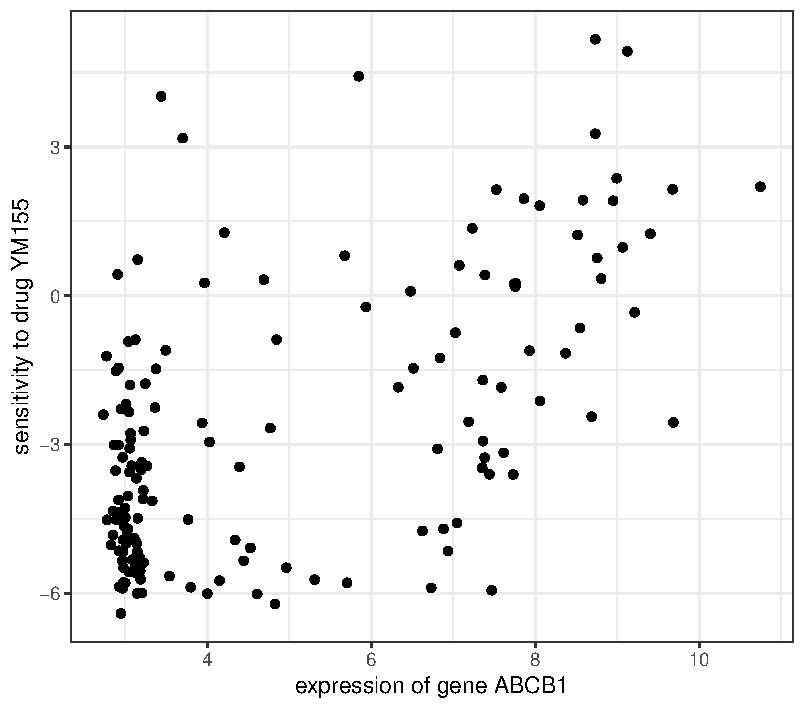
\includegraphics[height=6cm]{../figures/week_2_linear_models/Univariate_linear_regression_0.pdf}
\end{center}

\end{frame}

\begin{frame}
\frametitle{Example of univariate linear regression}
Least square fitting: linear function of $X$ that minimises the sum of squared residuals.

\begin{center}
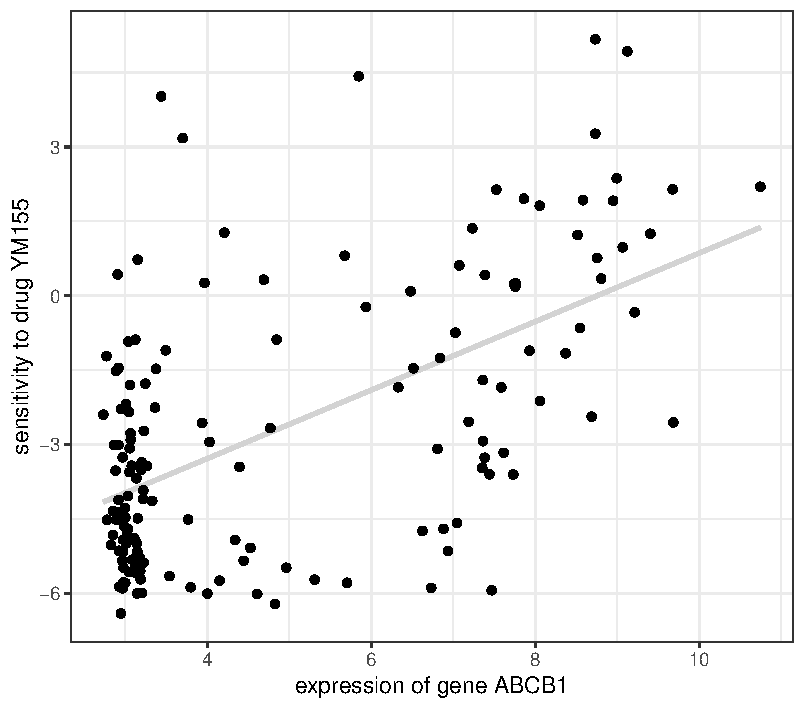
\includegraphics[height=6cm]{../figures/week_2_linear_models/Univariate_linear_regression_1.pdf}
\end{center}

\end{frame}

\begin{frame}
\frametitle{Example of univariate linear regression}
Least square fitting: linear function of $X$ that minimises the sum of squared residuals. $RSS = \sum_{i=1}^N (y_i - \beta_0 - \beta_1 x_i)^2$

\begin{center}
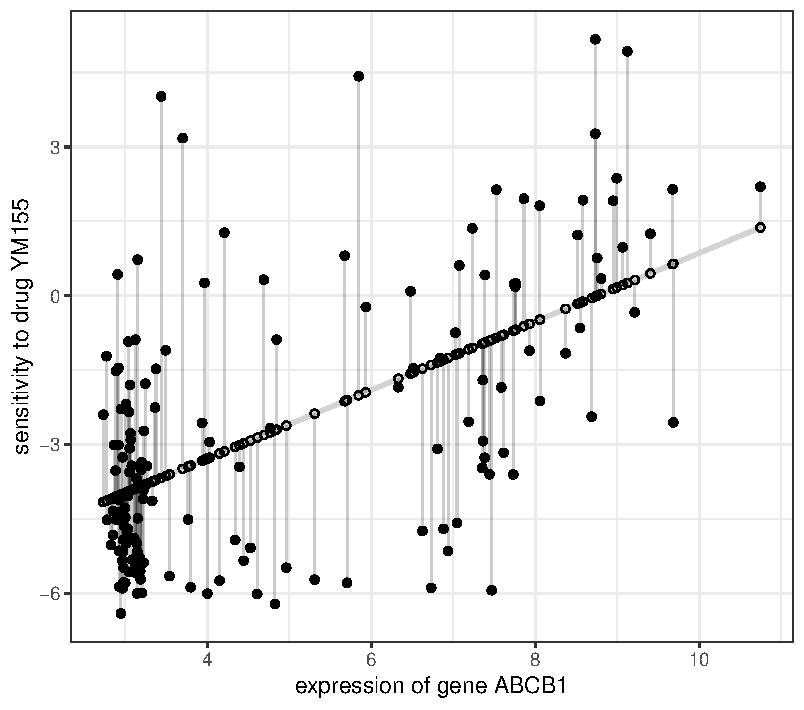
\includegraphics[height=6cm]{../figures/week_2_linear_models/Univariate_linear_regression_2.pdf}
\end{center}

\end{frame}

\begin{frame}
\frametitle{Genomics of Drug Sensitivity in Cancer (GDSC) project}
We will use as example data from the GDSC project (https://www.cancerrxgene.org/) \cite{GDSC}.

\begin{center}
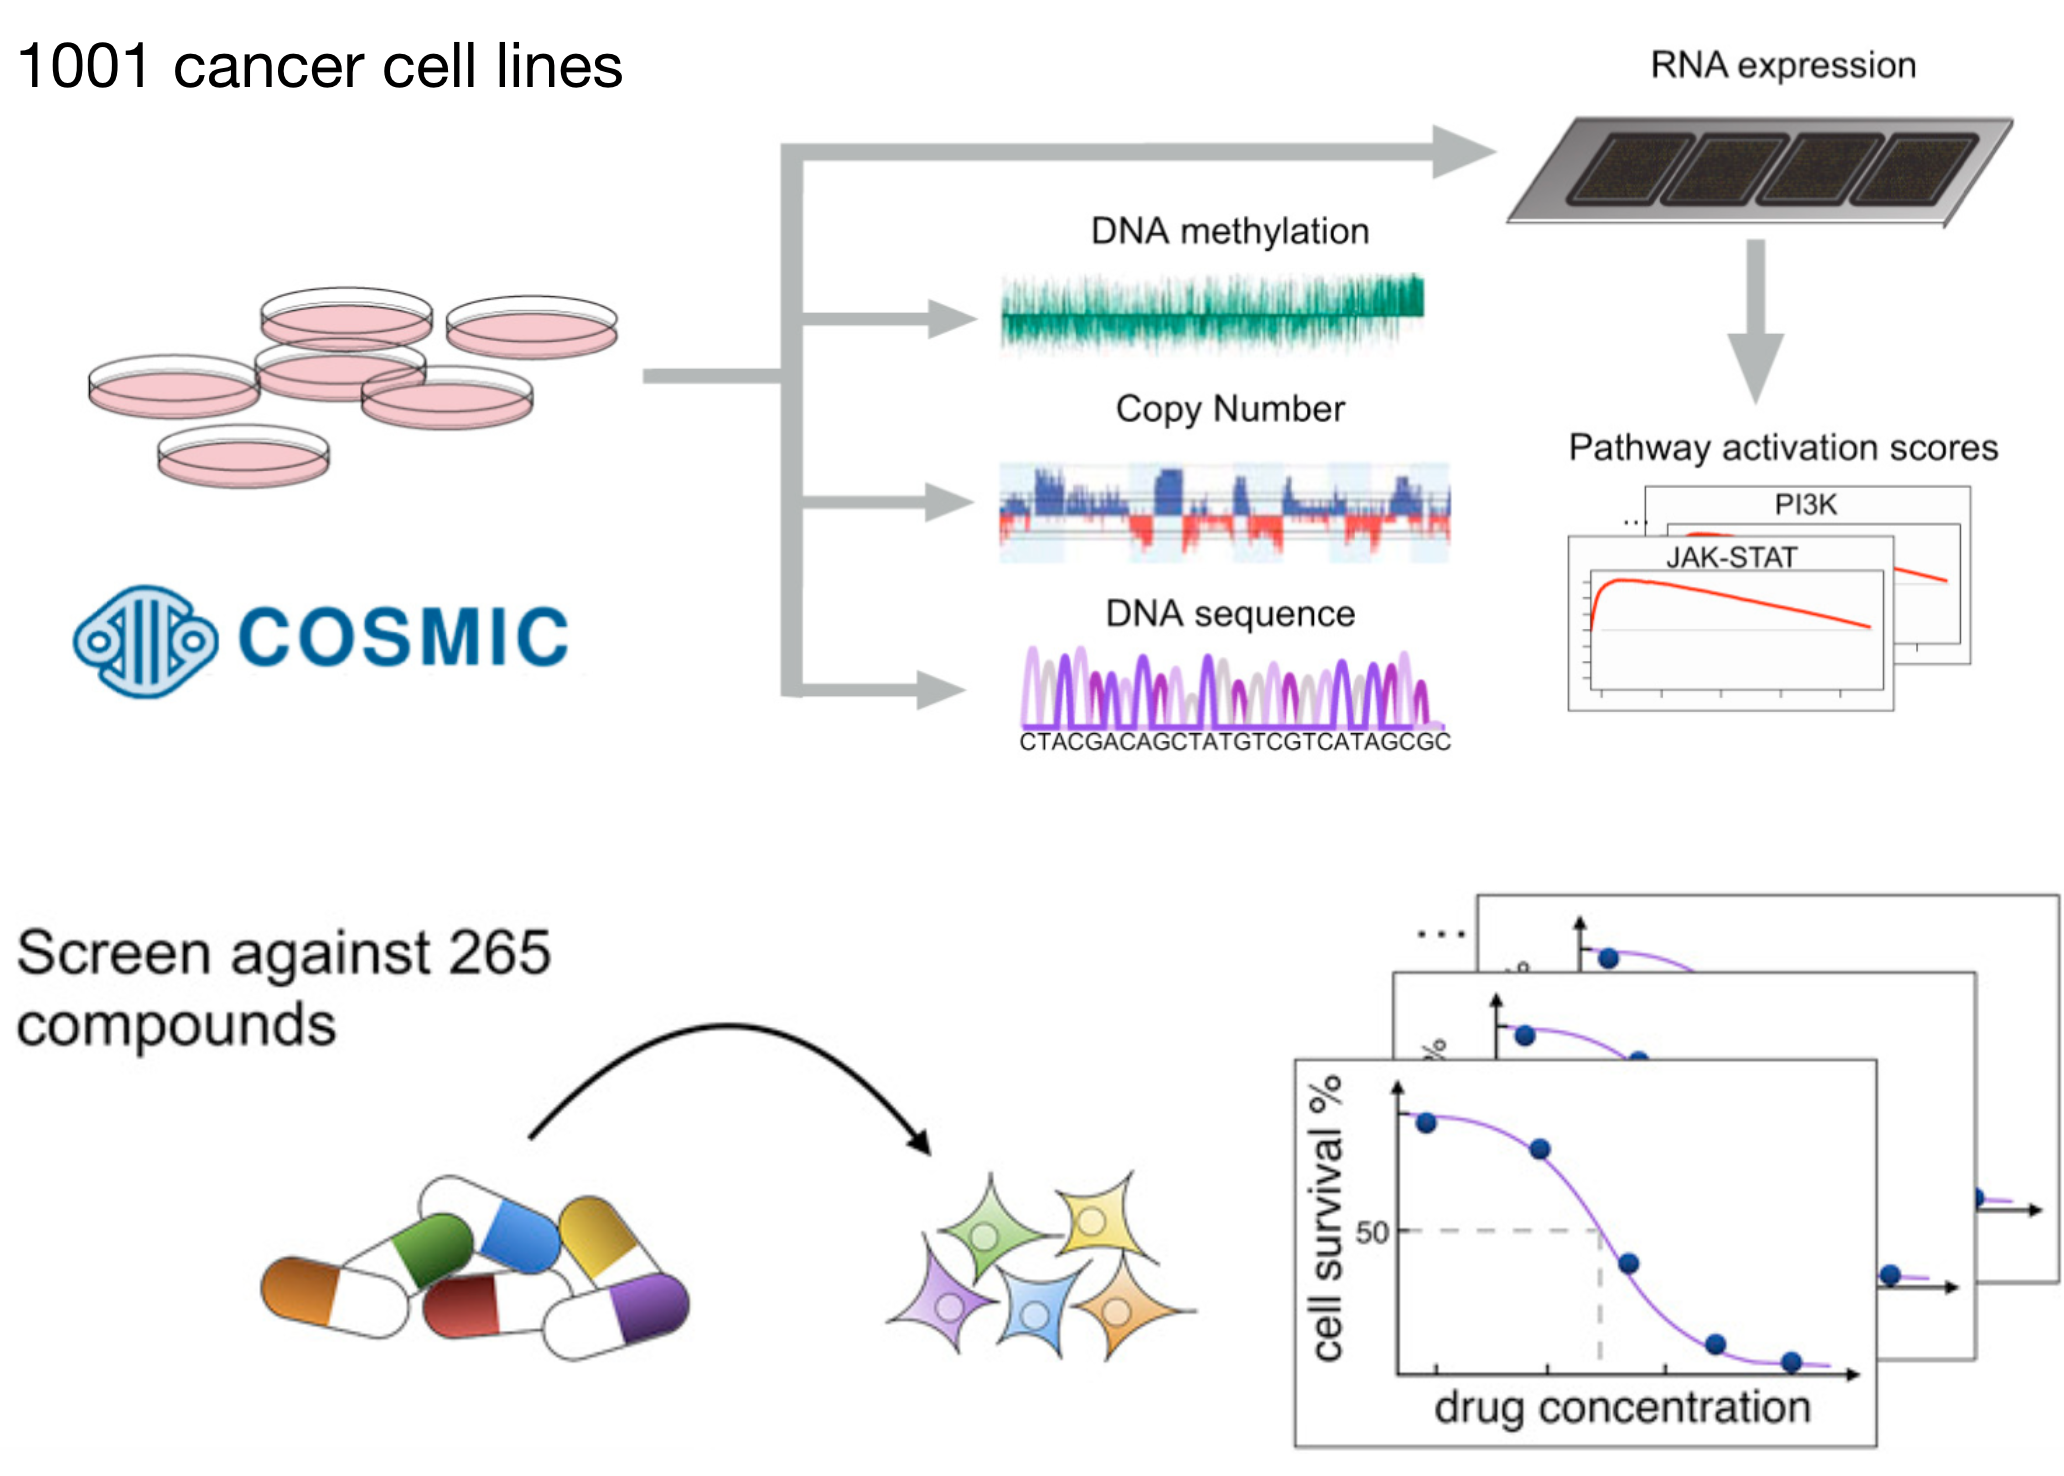
\includegraphics[height=6cm]{../figures/week_2_linear_models/GDSC_study_description.png}
\end{center}

\end{frame}

\begin{frame}
\frametitle{Genomics of Drug Sensitivity in Cancer (GDSC) project}
Cancer patients tends to respond very differently to drugs. A big challenge in cancer research 
is to find ways to assign the optimal treatment to each patient.

\begin{center}
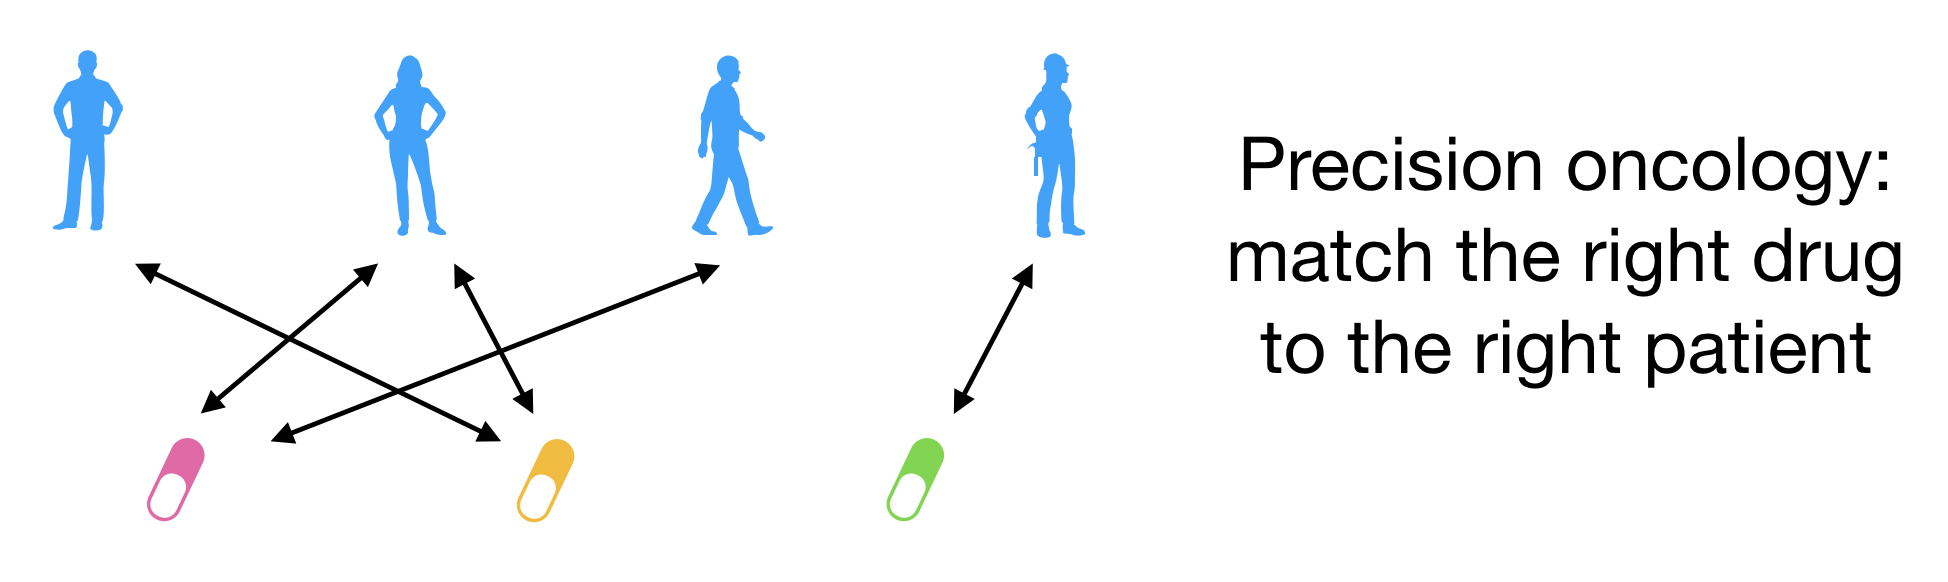
\includegraphics[height=2.5cm]{../figures/week_2_linear_models/precision_oncology.png}
\end{center}

The aim of the study is to find biomarkers of drug sensitivity.

\begin{center}
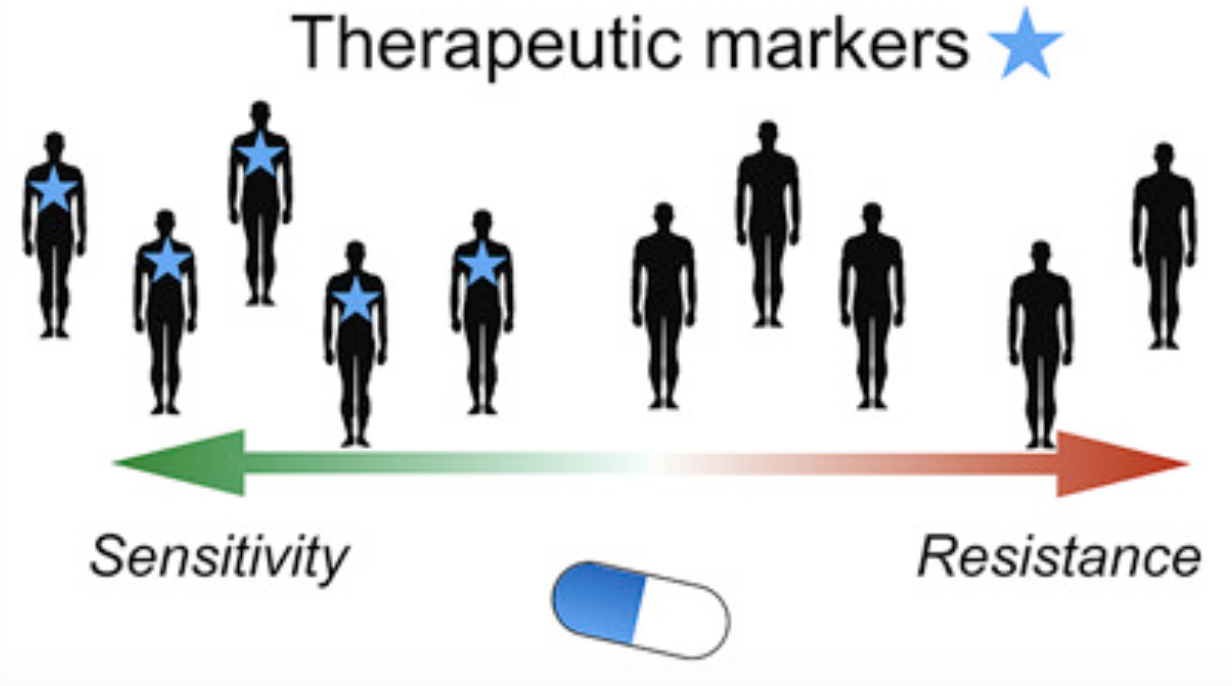
\includegraphics[height=2.5cm]{../figures/week_2_linear_models/GDSC_study_aim.png}
\end{center}

\end{frame}

\begin{frame}
\frametitle{Our dataset}

We will consider data for 148 cell lines from four cancer types.

\begin{center}
\begin{tabular}{ |c|c| } 
 \hline
 ID & Cancer type \\
 \hline
 COAD/READ & Colorectal adenocarcinoma \\ 
 NB & Neuroblastoma \\ 
 KIRC & Kidney renal clear cell carcinoma \\ 
 BRCA & Breast carcinoma \\
 \hline
\end{tabular}
\end{center}

We can interpret the prediction of drug sensitivity as a linear regression problem using:

\begin{itemize}
    \item Output variable: Sensitivity to YM155 (Sepantronium bromide), as natural log of the fitted IC50. 
    \item Predictors: expression of 244 genes (the ones with higher variance), as RMA normalised expression.
\end{itemize}

\end{frame}

\begin{frame}
\frametitle{Feature scaling}

Idea: make sure features are on a similar scale.

\begin{equation*}
x_i = \frac{x_i-\mu_i}{\sigma_i}
\end{equation*}

where $\mu_i$ and $\sigma_i$ are respectively the average and the standard deviation of all the values of feature $i$.

\vspace{5mm}

This makes the estimated coefficients comparable and speeds up the optimization algorithm.

\vspace{5mm} 

If we standardize the predictors, the solution for $\hat{\beta_0}$ is $\overline{y}$, therefore we fit a model without the intercept.

\end{frame}


\section{Subset selection}

\begin{frame}
\frametitle{Model complexity}

Especially when we have a large number of features ($p$ large compared to $N$), least squares estimates can suffer from:

\begin{itemize}
    \item Low \textit{prediction accuracy}: high model complexity gives low bias but high variance, setting some coefficients to zero can reduce the variance of predictions (at the price of increasing the bias).
    \item Poor \textit{interpretability}: we might want to identify which predictors are really useful to explain the output.
\end{itemize}

\end{frame}


\begin{frame}
\frametitle{Mentimeter question (www.menti.com code 1702 7678)}

A model with a high number of parameters will tend to:
\begin{itemize}
    \item represent well the training set but not the test set
    \item represent well the test set but not the training set
    \item represent well both
\end{itemize}
\end{frame}


\begin{frame}
\frametitle{Model complexity and overfitting}

\begin{center}
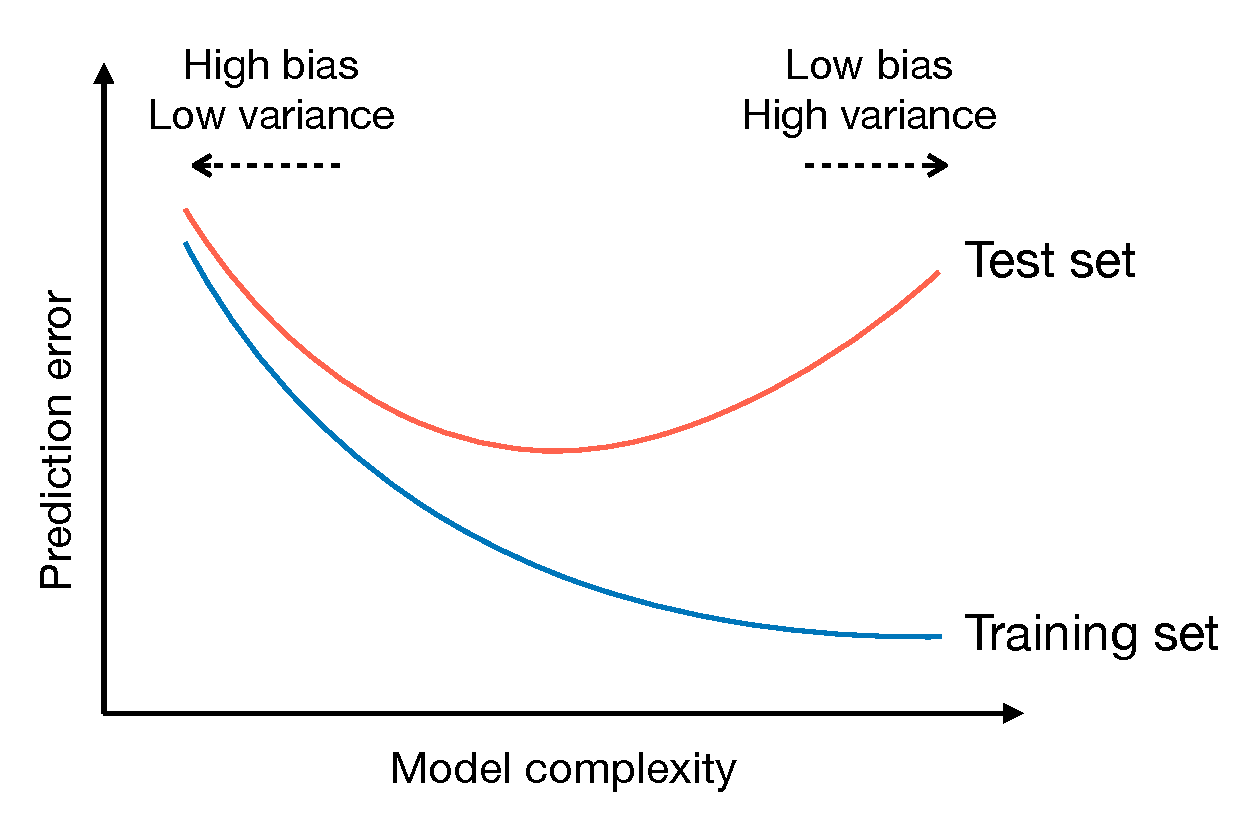
\includegraphics[height=5.5cm]{../figures/week_2_linear_models/Bias_variance_complexity.pdf}
\end{center}

Complex models tend to overfit the training data and perform poorly on the test data.

\end{frame}



\begin{frame}
\frametitle{Subset selection}

With \textit{subset selection} we want to retain only a subset of the predictors and eliminate the rest from the model.

\vspace{5mm} 

We can try a lot of different models, each containing a different subset of the predictors, and check which model is the best, e.g. based on \textit{Akaike information criterion (AIC)} or \textit{Bayesian information criterion (BIC)}.

\vspace{5mm} 

Problem: there are a total of $2^p$ models that contain subsets of p predictors!!

\end{frame}

\begin{frame}
\frametitle{Subset selection}

Three classical approaches to step-wise \textit{subset selection}:

\begin{itemize}
    \item \textit{Forward selection}. Start from the null model (i.e. only intercept) and sequentially add to the model the variable that gives lowest RSS (i.e. higest improvement of the fit).
    \item \textit{Backward selection}. Start with the full model (i.e. all variables) and sequentially remove the predictor with the largest p-value (i.e. lower impact on the fit).
    \item \textit{Mixed selection}. Alternation of forward and backward steps to add variables that improves RSS while maintaining the p-value below a certain threshold.
\end{itemize}

\end{frame}

\begin{frame}
\frametitle{Subset selection}

\textit{Subset selection} tends to:

\begin{itemize}
    \item improve \textit{interpretability}: only the most relevant predictors useful to explain the output are selected.
    \item still suffer from  low \textit{prediction accuracy}: high variance (discrete process in retaining and discarding predictors) often does not reduce prediction error.
\end{itemize}

\end{frame}


\section{Shrinkage methods}

\begin{frame}
\frametitle{Improving least square estimates with regularization}
\begin{itemize}
	\item least square estimates generally provide all non-zero coefficient.
	\item if $p>N$, solutions are not unique (i.e. multiple solutions with same minimum, often overfitting the data).
\end{itemize}


\vspace{5mm} 

Need to constrain or regularize the estimation process.

\vspace{5mm} 

Idea: shrink regression coefficients by imposing a penalty on their size.


\end{frame}

\begin{frame}
\frametitle{Ridge regression}
\textit{Ridge regression} penalizes the sum of squares of the coefficients (L2 regularization). 

\begin{align*}
\hat{\beta}^{ridge} &= \argmin_{\beta} \left\{ \sum_{i=1}^N (y_i - \beta_0 -  \sum_{j=1}^p x_{ij}\beta_j)^2 + \lambda \sum_{j=1}^p \beta_j^2 \right\} \\
& =  \argmin_{\beta} \left\{ RSS + \lambda \sum_{j=1}^p \beta_j^2 \right\}
\end{align*}

\end{frame}


\begin{frame}
\frametitle{Ridge regression: the meaning of $\lambda$}

\begin{equation*}
    \hat{\beta}^{ridge} =  \argmin_{\beta} \left\{ RSS + \lambda \sum_{j=1}^p \beta_j^2 \right\}
\end{equation*}

$\lambda \geq 0$ is a tuning parameter.

\begin{itemize}
    \item $\lambda = 0$ corresponds to the least square estimates.
    \item for larger values of $\lambda$, coefficients $\beta_1, \dots, \beta_p$ will be shrinked towards zero
\end{itemize}
\end{frame}

\begin{frame}
\frametitle{Ridge regression: the meaning of $\lambda$}


\begin{center}

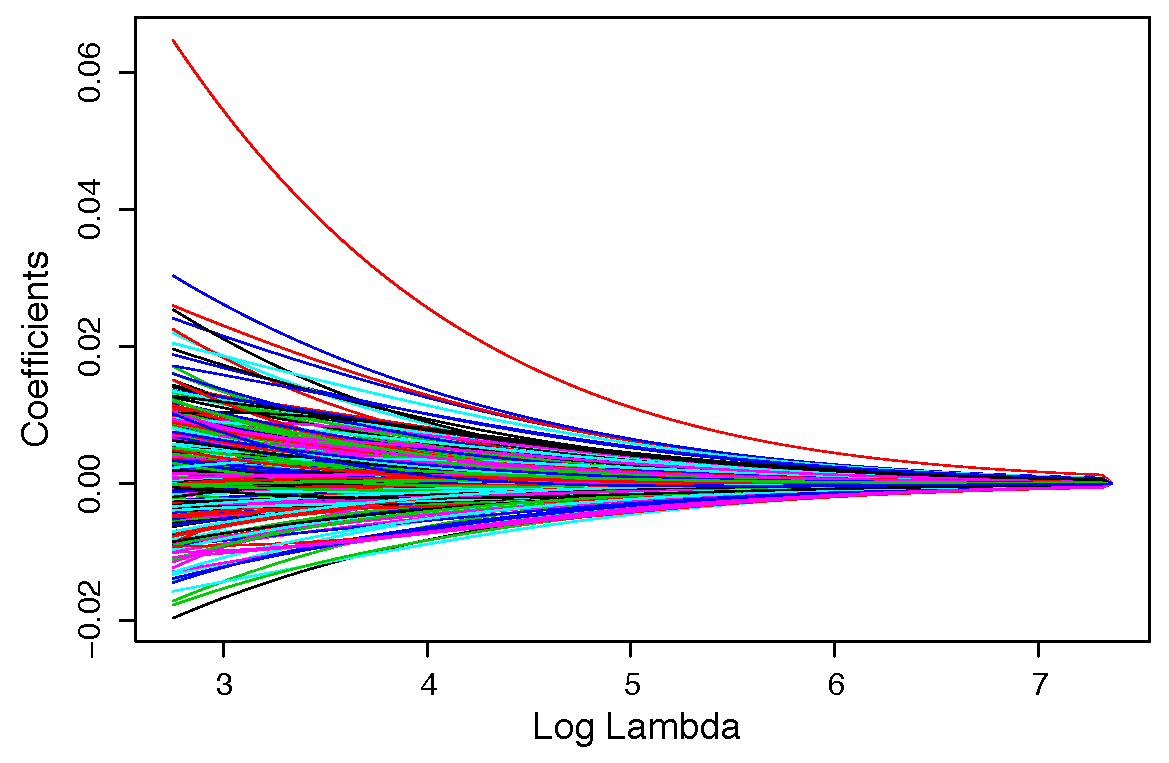
\includegraphics[height=5.5cm]{../figures/week_2_linear_models/Ridge_regression_coefficinets.pdf}
\end{center}

Profile of the Ridge regression coefficients for the GDSC example.

\end{frame}

\begin{frame}
\frametitle{The effect of regularization on bias and variance}
In matrix form we can rewrite the Ridge regression as:

\begin{equation*}
    (\mathbf{y} - \mathbf{X}\beta)^T (\mathbf{y} - \mathbf{X}\beta) + \lambda\beta^T\beta
\end{equation*}

And the Ridge regression solution becomes:

\begin{equation*}
    \hat{\beta}^{ridge} = (\mathbf{X}^T \mathbf{X} + \lambda \mathbf{I})^{-1}\mathbf{X}^T\mathbf{y} 
\end{equation*}

where $\mathbf{I}$ is the $p \times p$ identity matrix. This is linear in $\mathbf{y}$ and in closed form.

Assuming that $\mathbf{y} = \mathbf{X}\beta_{\mathrm{true}} + \mathbf{e}$, where $\mathbf{e}$ is a random error on the output variable, the Ridge regression solution can be written as:

\begin{align*}
    \hat{\beta}^{ridge} &= (\mathbf{X}^T \mathbf{X} + \lambda \mathbf{I})^{-1}\mathbf{X}^T(\mathbf{X}\beta_{\mathrm{true}} + \mathbf{e}) \\
    &= \underbrace{(\mathbf{X}^T \mathbf{X} + \lambda \mathbf{I})^{-1}\mathbf{X}^T\mathbf{X}\beta_{\mathrm{true}}}_{\textrm{bias}} + \underbrace{(\mathbf{X}^T \mathbf{X} + \lambda \mathbf{I})^{-1}\mathbf{X}^T\mathbf{e}}_{\textrm{variance}}
\end{align*}

\end{frame}

\begin{frame}
\frametitle{Mentimeter question (www.menti.com code 1702 7678)}

What is the value of $\lambda$ that gives the minimum variance?

\end{frame}


\begin{frame}
\frametitle{The effect of regularization on bias and variance}
Effect of $\lambda$ on the bias-variance trade off in a simulated example ($y_i = x_{i1}\beta_1 + x_{i2}\beta_2 + e_i$, $i=1,\dots, 20$). The model is simulated 50k times, each time the noise $e_i$ is randomly generated.




\begin{center}
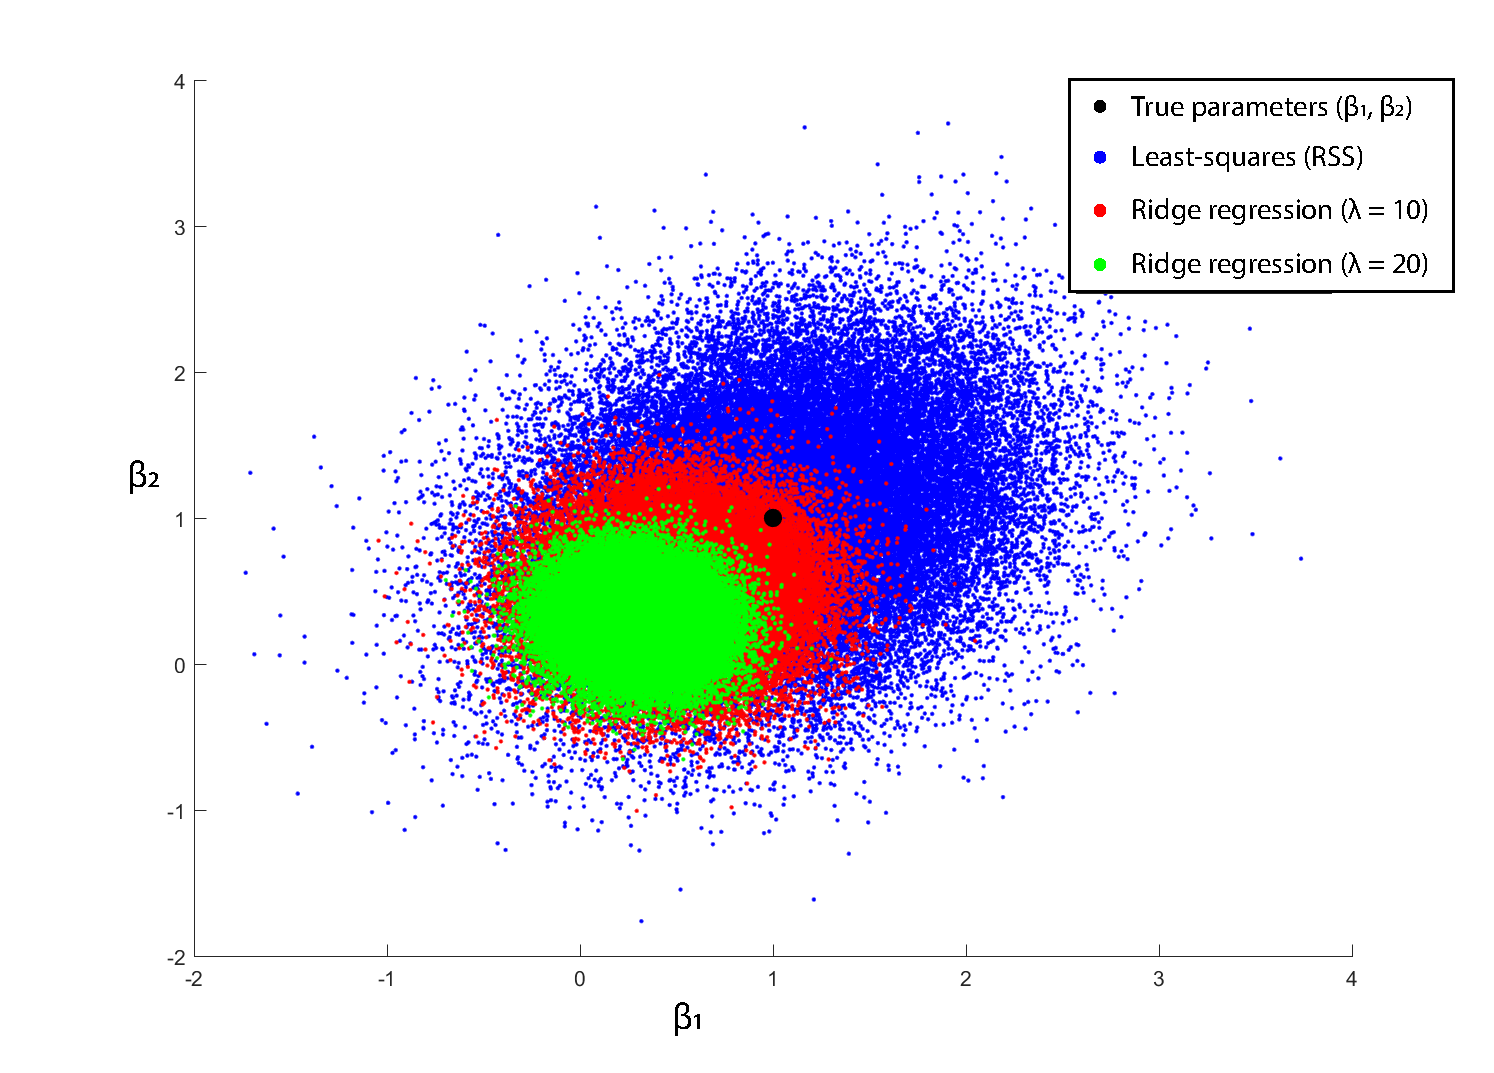
\includegraphics[height=5.5cm]{../figures/week_2_linear_models/Ridge_bias_variance_insilico.pdf}
\end{center}

\end{frame}


\begin{frame}
\frametitle{Lasso regression}
\textit{Lasso regression} penalizes the sum of the absolute value of the coefficients (L1 regularization). 

\begin{align*}
\hat{\beta}^{lasso} &= \argmin_{\beta} \left\{ \sum_{i=1}^N (y_i - \beta_0 -  \sum_{j=1}^p x_{ij}\beta_j)^2 + \lambda \sum_{j=1}^p | \beta_j | \right\} \\
& =  \argmin_{\beta} \left\{ RSS + \lambda \sum_{j=1}^p | \beta_j | \right\}
\end{align*}

\end{frame}


\begin{frame}
\frametitle{Lasso regression: the meaning of $\lambda$}

\begin{equation*}
    \hat{\beta}^{lasso} =  \argmin_{\beta} \left\{ RSS + \lambda \sum_{j=1}^p | \beta_j | \right\}
\end{equation*}

$\lambda \geq 0$ is a tuning parameter.

\begin{itemize}
    \item $\lambda = 0$ corresponds to the least square estimates
    \item larger values of $\lambda$, will make some of the coefficients $\beta_1, \dots, \beta_p$ to be exactly zero, performing a continuous subset selection.
\end{itemize}
\end{frame}

\begin{frame}
\frametitle{Mentimeter question (www.menti.com code 1702 7678)}

A high value of $\lambda$:
\begin{itemize}
    \item increases model complexity
    \item reduces model complexity
    \item doesn't affect model complexity
\end{itemize}
\end{frame}



\begin{frame}
\frametitle{Lasso regression: the meaning of $\lambda$}

\begin{center}
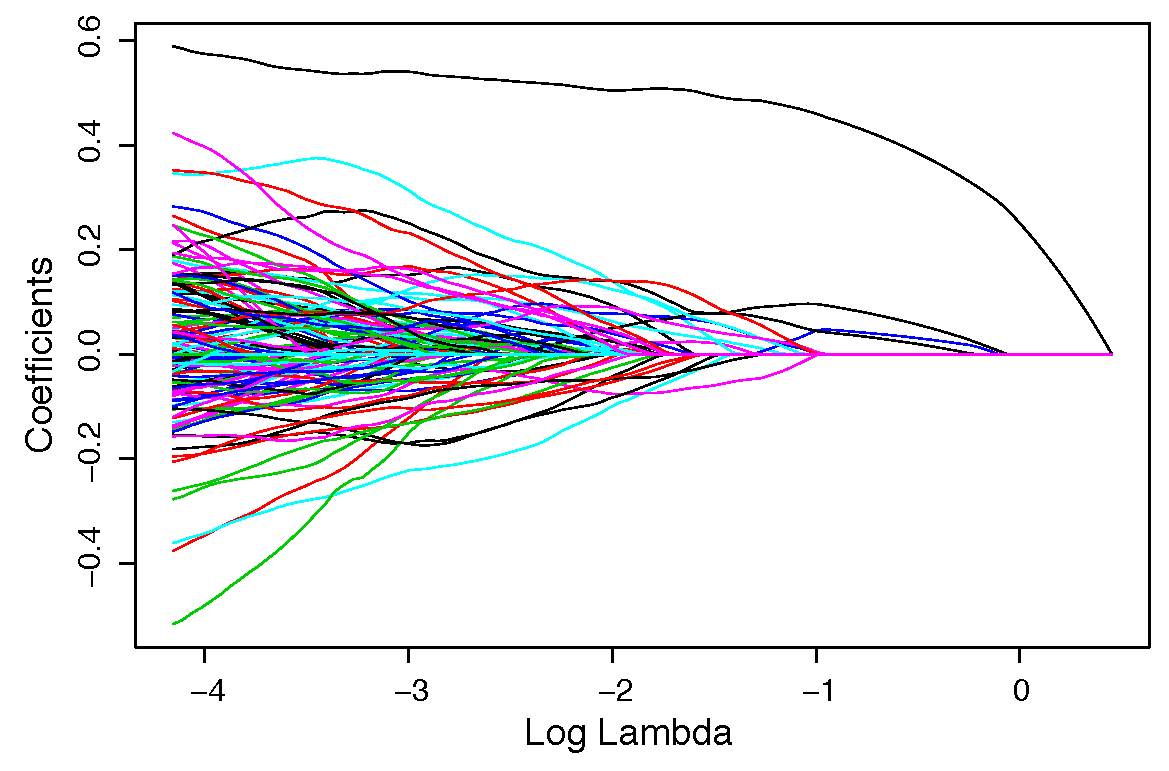
\includegraphics[height=5.5cm]{../figures/week_2_linear_models/Lasso_regression_coefficinets.pdf}
\end{center}

Profile of the Lasso regression coefficients for the GDSC example.

\end{frame}

\begin{frame}
\frametitle{Comparing Lasso and Ridge regression}

An equivalent way or writing the Ridge and Lasso problems is:

\begin{equation*}
    \argmin_{\beta} \sum_{i=1}^N (y_i - \beta_0 -  \sum_{j=1}^p x_{ij}\beta_j)^2
\end{equation*}

subject to: 
\begin{itemize}
    \item $\sum_{j=1}^p \beta_j^2 < t$ for Ridge regression
    \item $\sum_{j=1}^p | \beta_j | < t$ for Lasso regression
\end{itemize}

\vspace{5mm} 

It is possible to show that there is a one-to-one correspondence between the parameter $\lambda$ and $t$.

\end{frame}


\begin{frame}
\frametitle{Comparing Lasso and Ridge regression}

\begin{center}
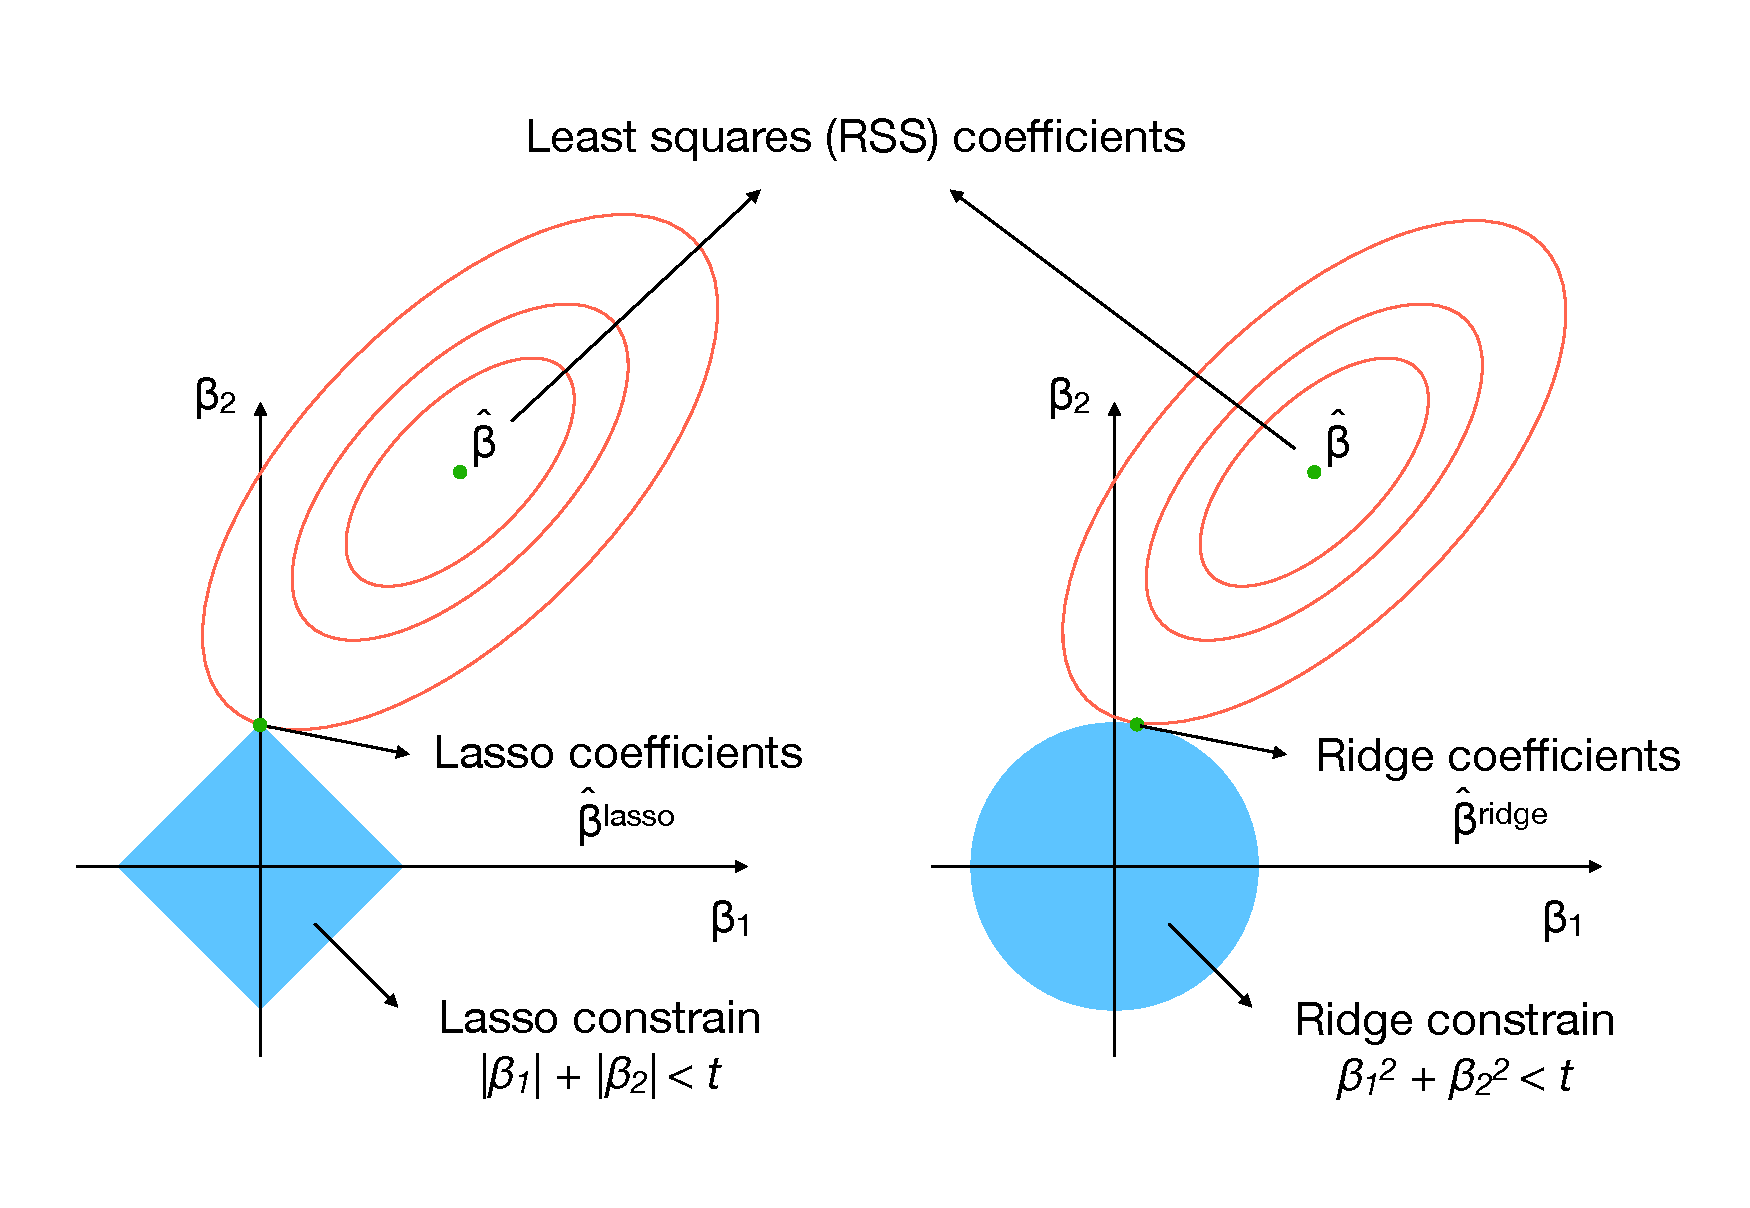
\includegraphics[height=7cm]{../figures/week_2_linear_models/Comparison_lasso_ridge.pdf}
\end{center}

\end{frame}


\begin{frame}
\frametitle{How to select optimal $\lambda$}

We need a method to select the tuning parameter $\lambda$ for both Lasso and Ridge regression.

\vspace{5mm} 

We want the model that provides the best predictions on the test set. In general this is very sensitive to the data used for training.
\end{frame}


\begin{frame}
\frametitle{How to select optimal $\lambda$}

Two data partitions - GDSC example (90\% training, 10\% test).

\begin{center}
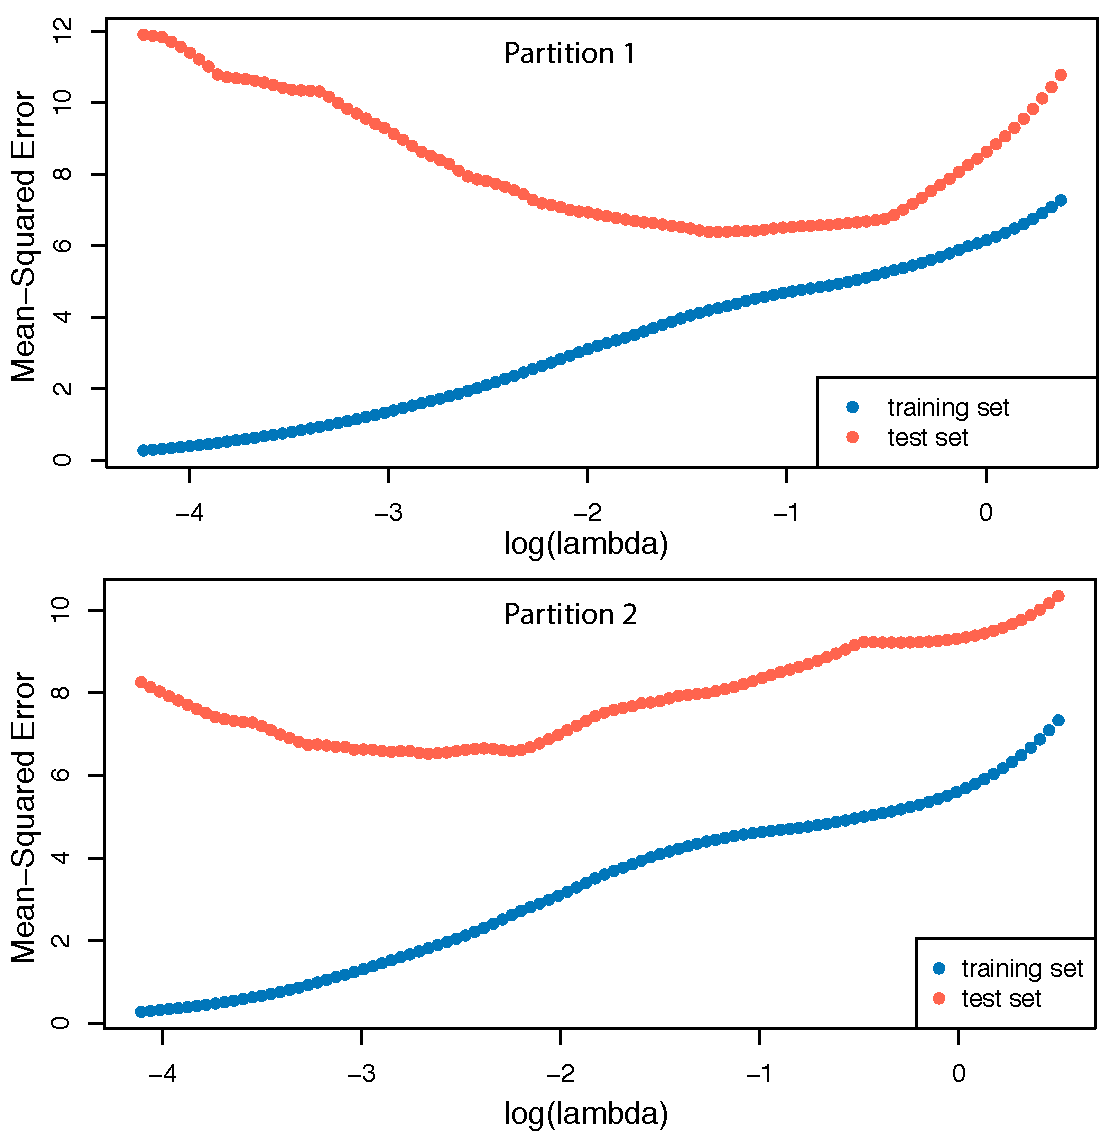
\includegraphics[height=7cm]{../figures/week_2_linear_models/Lasso_MSE_train_test.pdf}
\end{center}
\end{frame}

\begin{frame}
\frametitle{How to select optimal $\lambda$}

We can use cross-validation following these steps:
\begin{enumerate}
  \item Choose a grid of $\lambda$.
  \item Optimize the model for each training set and compute Mean-Squared Error (MSE) for each validation set.
  \item Choose the model with smallest cross-validation error.
  \item Re-fit using all the available observations and the selected tuning parameter.
\end{enumerate}

\end{frame}

\begin{frame}
\frametitle{$\lambda$ selection: GDSC example 10-fold cross validation}

\begin{center}
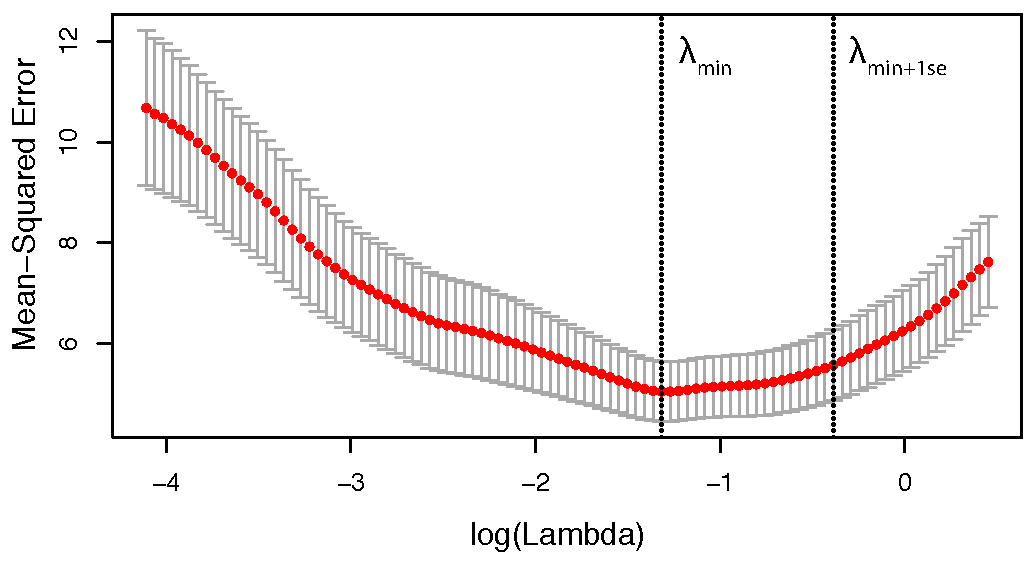
\includegraphics[height=5cm]{../figures/week_2_linear_models/Lasso_MSE_crossvalidation.pdf}
\end{center}

\vspace{-2mm} 

\begin{itemize}
    \item $\lambda_{min}$: value of $\lambda$ that gives the minimum MSE
    \item $\lambda_{min+1se}$: largest value of $\lambda$ such that error is within 1 standard error of the minimum
\end{itemize}

\end{frame}

\begin{frame}
\frametitle{Mentimeter question (www.menti.com code 1702 7678)}

Would you select $\lambda_{min}$ or $\lambda_{min+1se}$ to have a less complex model'?

\end{frame}

\begin{frame}
\frametitle{Lasso for feature selection}
GDSC example 10-fold cross validation

\begin{center}
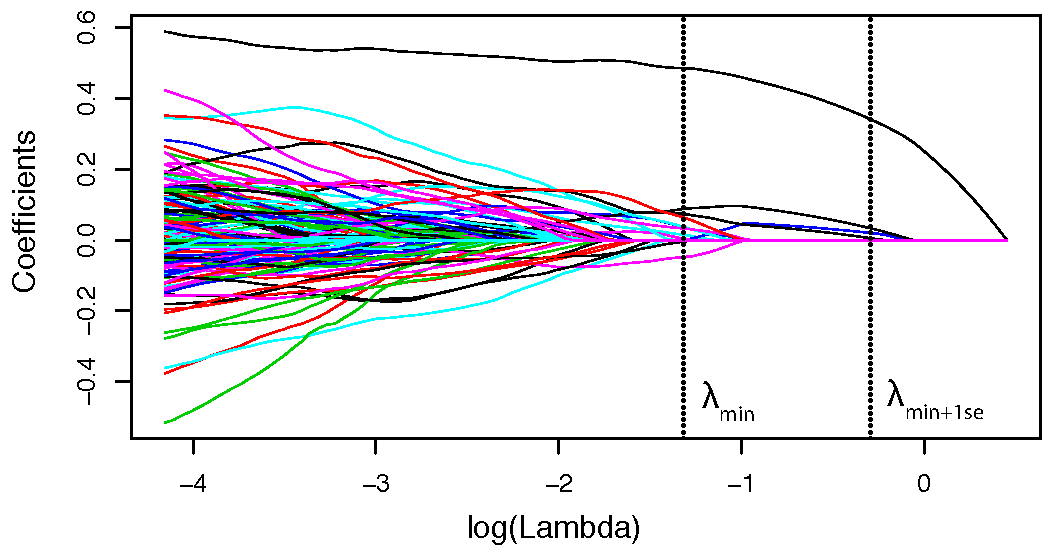
\includegraphics[height=5cm]{../figures/week_2_linear_models/Lasso_feature_selection.pdf}
\end{center}

$\lambda_{min+1se}$ gives more sparse solutions.

\end{frame}


\begin{frame}
\frametitle{Lasso for feature selection}

Selected features can be sensitive to the partition of the cross-validation.

\vspace{5mm} 

To select only robust features we can use \textit{bootstrap}: feature selection procedure is repeated M times, using every time a different bootstrapped dataset (i.e. sampling N samples with replacement).

\end{frame}


\begin{frame}
\frametitle{Lasso for feature selection: using bootstrap}
GDSC example: 100 times bootstrap (with 10-fold cross-validation)

\begin{center}
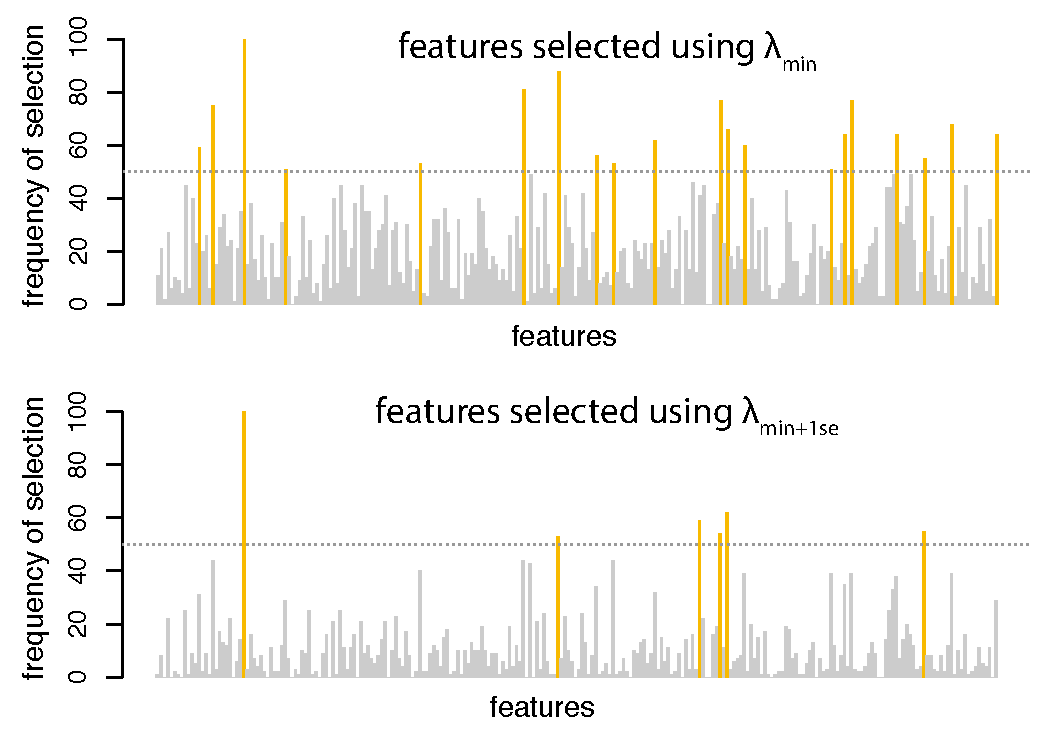
\includegraphics[height=7cm]{../figures/week_2_linear_models/Lasso_feature_selection_bootstrap.pdf}
\end{center}

\end{frame}




\begin{frame}
\frametitle{Collinearity}
Two or more predictor variables can be closely related to each other and show a high correlation.

\vspace{5mm} 

This is common in genomic data, because genes can be redundant or have related functions.

\begin{center}
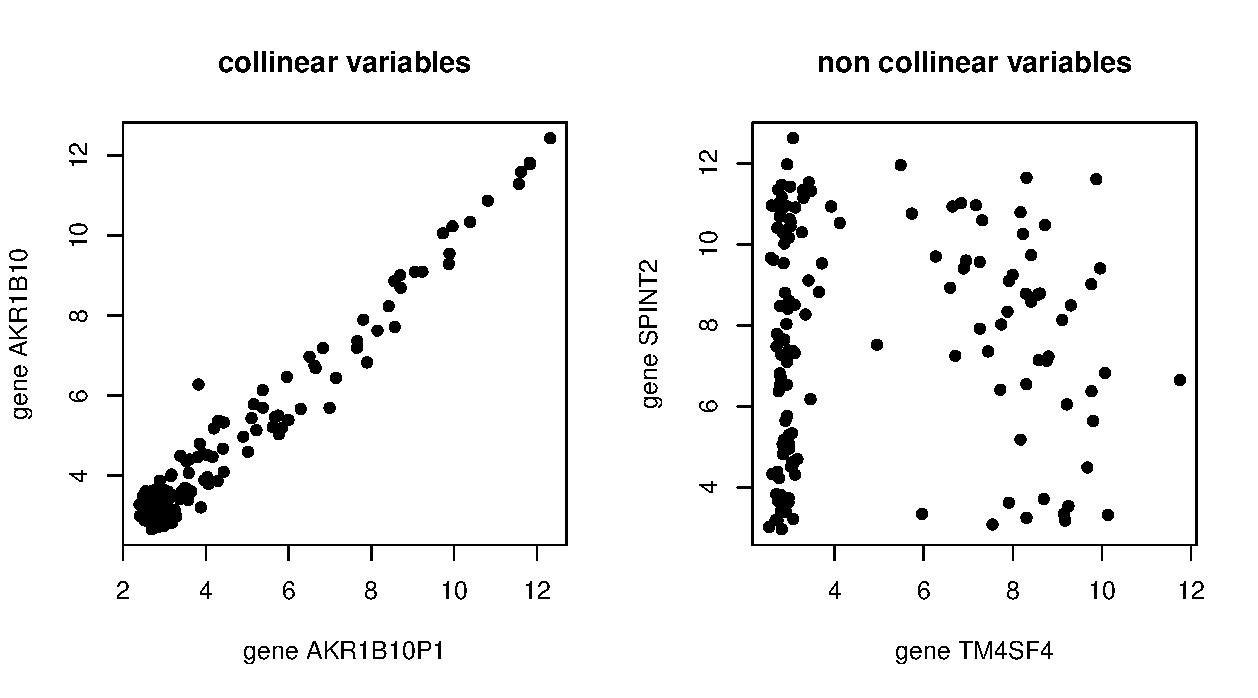
\includegraphics[height=5cm]{../figures/week_2_linear_models/collinearity.pdf}
\end{center}

\end{frame}

\begin{frame}
\frametitle{Collinearity}
The effect of \textit{collinear variables} can be difficult to separate in the regression context.

\vspace{5mm} 

\textit{Collinearity} in general reduces the accuracy of the estimates of the coefficients of the correlated variables.

\vspace{5mm} 

When using Lasso, \textit{collinearity} can result in an arbitrary selection of one or the other correlated feature, depending on the data used for training.
\end{frame}

\begin{frame}
\frametitle{Mentimeter question (www.menti.com code 1702 7678)}

If you do bootstrap with lasso with 2 explanatory features which are collinear, what do you expect as frequency of selection?

\end{frame}

\begin{frame}
\frametitle{Elastic Net regression}

Elastic Net provides a compromise between Ridge and Lasso, by selecting variables like Lasso and shrinking together correlated variables like Elastic Net.


\begin{equation*}
    \hat{\beta}^{elastic net} =  \argmin_{\beta} \left\{ RSS + \lambda \sum_{j=1}^p ((\alpha \beta_j^2 + (1-\alpha)| \beta_j |) \right\}
\end{equation*}

Where $\alpha$ is a tunable parameter. This corresponds to:

\begin{itemize}
    \item Ridge for $\alpha=1$
    \item Lasso for $\alpha=0$
\end{itemize}

\end{frame}

\begin{frame}
\frametitle{Elastic Net regression}

\begin{center}
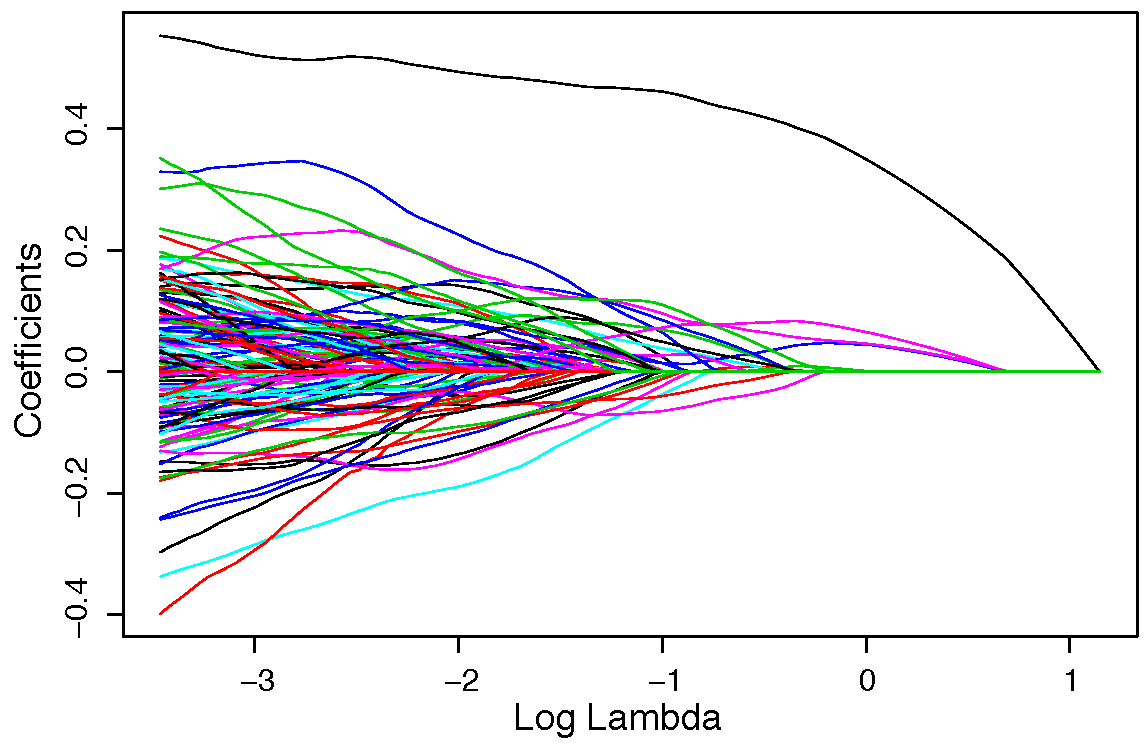
\includegraphics[height=5.5cm]{../figures/week_2_linear_models/ElasticNet_regression_coefficinets.pdf}
\end{center}

Profile of the Elastic net (with $\alpha=0.5$) regression coefficients for the GDSC example.

\end{frame}

\section{Classification}

\begin{frame}
\frametitle{Classification}
In a clinical setting, instead of predicting the continuous IC50 for each patient, we might be interested in classifying patients in sensitive or resistant to a specific drug.

\vspace{5mm} 

Using the cell lines from the GDSC study this corresponds to divide them in sensitive and resistant to the drug. 

\begin{center}
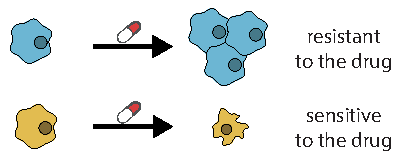
\includegraphics[height=2.7cm]{../figures/week_2_linear_models/GDSC_classification_overview.pdf}
\end{center}

Cell lines are separated in sensitive and resistant based on the average response across all cell lines in the panel.

\end{frame}

\begin{frame}
\frametitle{Classification}

For binary classification we will consider a positive and a negative class:

\begin{itemize}
    \item 0 ("negative class"): sensitive
    \item 1 ("positive class"): resistant
\end{itemize}

\begin{center}
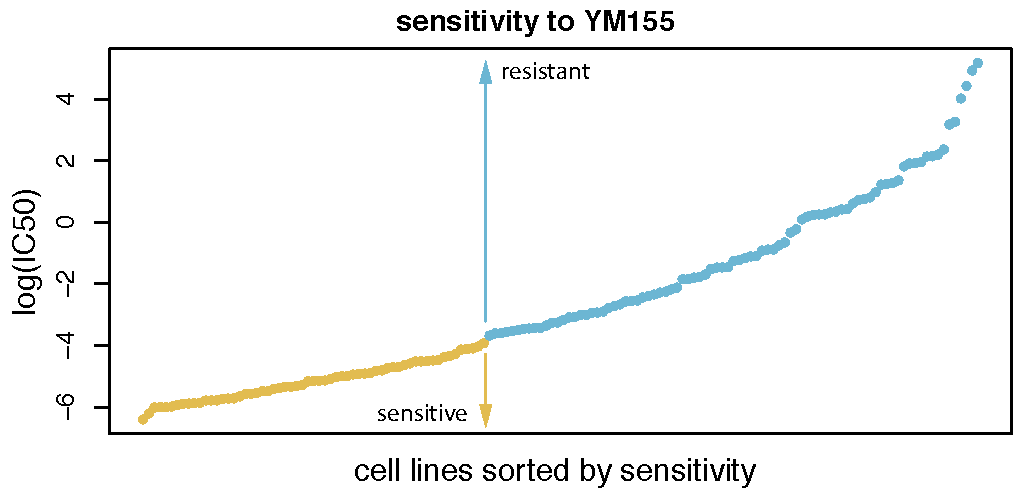
\includegraphics[height=5cm]{../figures/week_2_linear_models/GDSC_classification_sensitivity.pdf}
\end{center}
\end{frame}


\begin{frame}
\frametitle{Example of classification with one variable}

Using the same example used for univariate linear regression, we consider the ability of gene ABCB1 to classify cell lines in sensitive and resistant.

\begin{center}
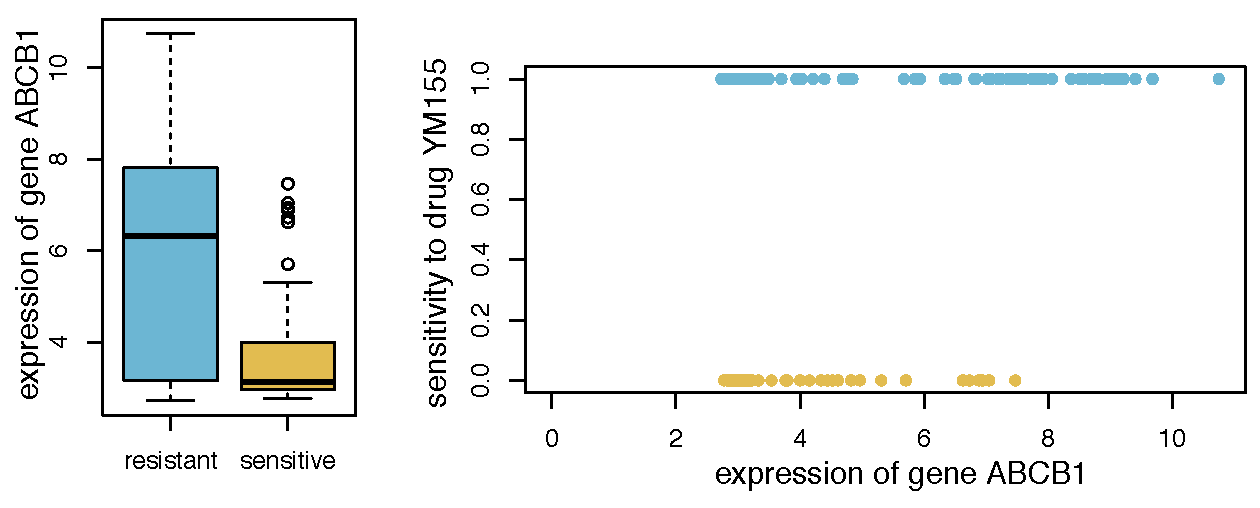
\includegraphics[height=4cm]{../figures/week_2_linear_models/GDSC_one_variable_example_logistic_regression_1.pdf}
\end{center}

\end{frame}

\begin{frame}
\frametitle{Example of classification with one variable}

We can try to fit a linear regression to a binary response, e.g.using 0.5 as threshold for prediction.

\begin{center}
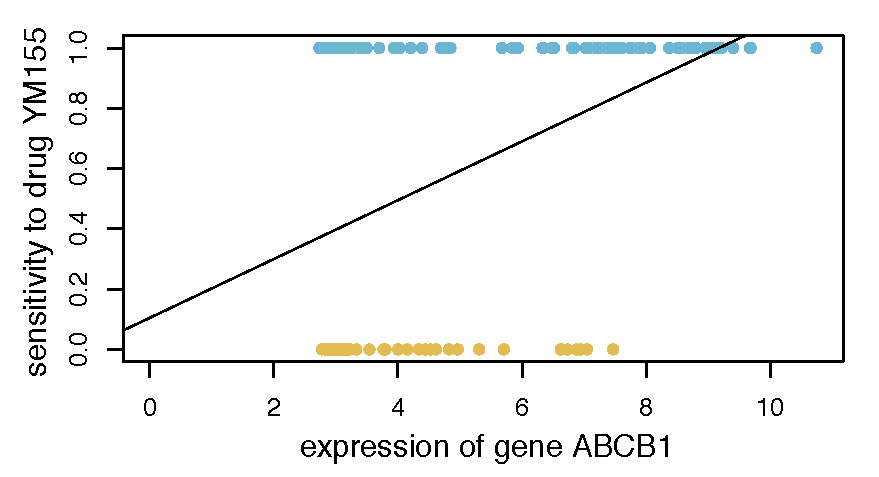
\includegraphics[height=4.5cm]{../figures/week_2_linear_models/GDSC_one_variable_example_logistic_regression_2.pdf}
\end{center}

Poor interpretability, with predicted values also outside [0, 1].

\end{frame}

\begin{frame}
\frametitle{Example of classification with one variable}

With logistic regression we want to model the probability (between 0 and 1) that $Y$ belongs to a particular class.

\begin{equation*}
Pr(response = resistant|ABCB1expression)
\end{equation*}


\begin{center}
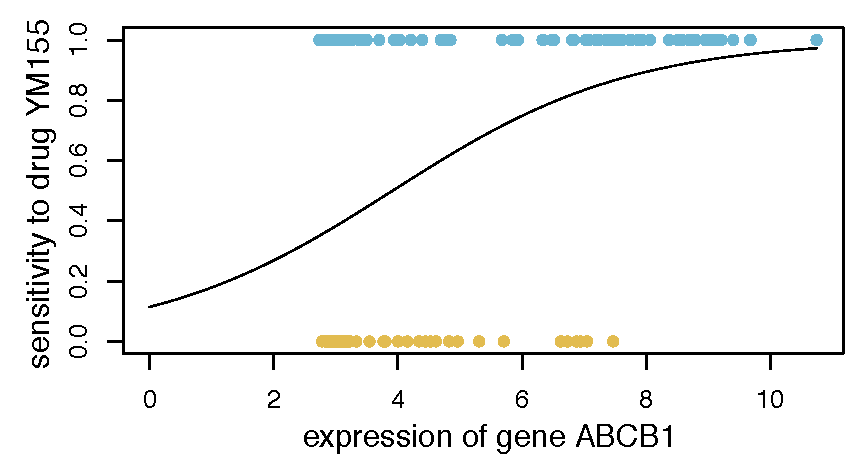
\includegraphics[height=4.5cm]{../figures/week_2_linear_models/GDSC_one_variable_example_logistic_regression_3.pdf}
\end{center}

\end{frame}


\section{Logistic regression}
\begin{frame}
\frametitle{Logistic regression}

\begin{equation*}
p(X) = Pr(G = 1|X)
\end{equation*}

With \textit{logistic regression} this probability is modeled as a \textit{logistic function}:

\begin{equation*}
p(X) = \frac{e^{\beta_0 + \beta_1X}}{1+e^{\beta_0 + \beta_1X}}
\end{equation*}

This corresponds to:

\begin{equation*}
\log \left(\frac{p(X)}{1-p(X)}\right)  = \beta_0 + \beta_1X
\end{equation*}

The left-hand side is called the log-odds or logit transformation and it is linear in X.

\end{frame}

\begin{frame}
\frametitle{Logistic regression: multi-class classification}

When having $K$ classes, the posterior probability is modeled as:

\begin{align*}
\log \frac{Pr(G=1 | X=x)}{Pr(G=K | X=x)} &= \beta_{10} + \beta_1^T x \\
\log \frac{Pr(G=2 | X=x)}{Pr(G=K | X=x)} &= \beta_{20} + \beta_2^T x \\
 & \vdots \\
\log \frac{Pr(G=K-1 | X=x)}{Pr(G=K | X=x)} &= \beta_{(K-1)0} + \beta_{K-1}^T x \\
\end{align*}

Using $K$-1 log-odds satisfies the constraint that probabilities sum to one. The choice of the last class to be used at denominator is arbitrary and does not affect the result.

\end{frame}



\begin{frame}
\frametitle{Logistic regression: parameters estimation}

The parameters for logistic regression models are generally estimated using \textit{maximum-likelihood}.

\vspace{5mm} 

\vspace{5mm} 

For $N$ observations the log-likelihood to be maximized is:

\begin{equation*}
    \ell(\theta) = \sum_{i=1}^N \log p_{g_i}(x_i; \theta)
\end{equation*}

where $p_k(x_i; \theta) = Pr(G=k|X=x_i; \theta)$ and $\theta$ is the parameter set.


\end{frame}

\begin{frame}
\frametitle{Logistic regression: parameters estimation}

For the two classes case, the response $y_i \in \{0,1\}$. Being $p(x_i;\beta)$ the probability for class 1, and $1-p(x_i;\beta)$ the probability for class 0, the log-likelihood can be written as:

\begin{align*}
    \ell(\beta) &= \sum_{i=1}^N \{ y_i \log p(x_i;\beta) + (1-y_i) \log (1-p(x_i;\beta)) \} \\
    &= \sum_{i=1}^N \{ y_i \beta^T x_i - \log (1+e^{\beta^T x_i}) \}
\end{align*}

where $\beta=\{ \beta_{10}, \beta_1\}$ and the vector of inputs $x_i$ includes the constant term 1 for the intercept.


\end{frame}



\begin{frame}
\frametitle{L1 regularized logistic regression}

Similarly to what we have seen for linear regression, regularization can be used for variable selection and shrinkage also with logistic regression.

\vspace{5mm} 

When applying L1 penalty we want to maximise a penalized version of the log-likelihood

\begin{equation*}
    \max_{\beta_0, \beta} \left\{ \sum_{i=1}^N [ y_i(\beta_0 + \beta^T x_i) - \log (1+e^{(\beta_0 + \beta^T x_i))}] -\lambda \sum_{j=1}^p | \beta_j| \right\}
\end{equation*}

Note that the intercept term is not penalized. Similarly to Lasso, the predictors should be standardized in order for the coefficients to be comparable.

\end{frame}

\begin{frame}
\frametitle{Example cross-validation}

Also in this case cross-validation can be used to select the tuning parameter.

\begin{center}
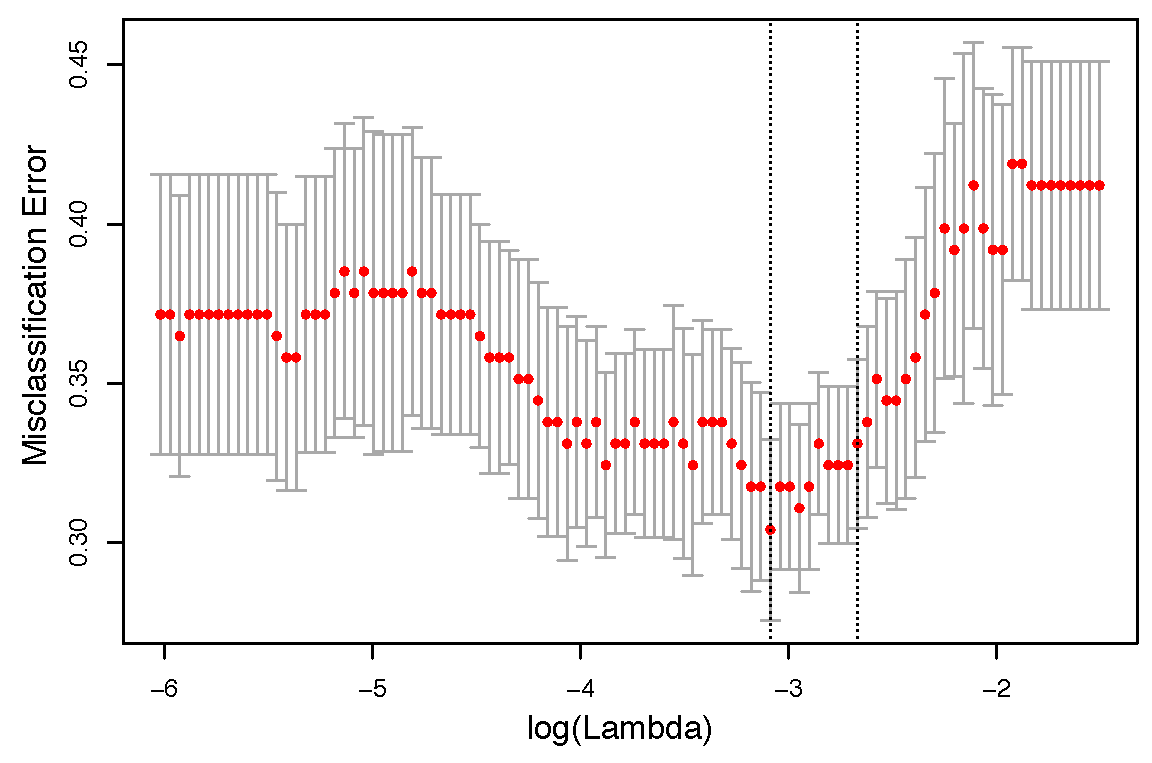
\includegraphics[height=4.5cm]{../figures/week_2_linear_models/GDSC_logistic_regression_cross_validation.pdf}
\end{center}

\end{frame}


\begin{frame}
\frametitle{References}
\printbibliography
\end{frame}


\end{document}
